% Use a modified ACM conference proceedings template
\documentclass[sigconf]{acmart}
% Disable some elements from ACM template
\setcopyright{none}
\settopmatter{printacmref=false,printfolios=false}

\usepackage{booktabs} % For formal tables
\usepackage[ruled,vlined]{algorithm2e}
\usepackage{amsmath} % for writing algorithms
\newcommand{\todo}[1]{{\color{red}{#1}}}

\begin{document}
\title{Machine Perception Report}

\author{Fatjon Zogaj}\affiliation{}
\email{fzogaj@student.ethz.ch}

\author{Patrik Okanovic}\affiliation{}
\email{pokanovic@student.ethz.ch}

\author{Rafael Sterzinger}\affiliation{}
\email{rsterzinger@student.ethz.ch}

\begin{abstract}
    This paper compares a variety of different architectures and techniques
    for the challenge of monocular 3D human pose estimation challenge on the H36M~\cite{h36m_pami} dataset.
    We propose to make use of standard augmentation and occlusion~\cite{sarandi_synthetic_2018},
    volumetric heatmap regression~\cite{sun_integral_2018-1} in combination with a pretrained ResNext101~\cite{DBLP:journals/corr/XieGDTH16}
    backbone for the highest score.
    Human joints follow the underlying structure
    of a graph which is why we also examine Graph Convolutional Network~\cite{zhao2019gcn}
    which we combine with evolutionary training data~\cite{Li_2020_CVPR}.
    Our best ResNext101 backed model is able to achieve state of art.
%Briefly summarize your report here. This should include a description of the task you are solving, a summary of how you approach the task (i.e. your method), as well as a preview of the central result. The abstract should be short, i.e. 4-5 sentences. The rest of this template outlines a rough structure how you \emph{can} organize your report. It mentions all the components we would typically expect. It is a good idea to adhere these guidelines, but they are not binding, i.e., you are free to re-organize your report as you see fit.
\end{abstract}

\maketitle

\section{Introduction}
%In this section, introduce the task in a bit more detail. In the first paragraph, try to answer why the task is of interest at all and what makes it challenging. You may also discuss some related work here. For example, you can summarize how other researchers have addressed the problem and what might be the disadvantages of these works.

%In the second half of the introduction, describe your method. This should be more detailed than in the abstract. You can talk about how your method relates to existing work (e.g. it is a combination or extension of existing methods, what other papers were you inspired by, etc.). You should also state the central result here, and the key insight that made it possible to achieve this result.

Human pose estimation (HPE) from a single monocular image is an open challenge garnering significant attention in computer vision ~\cite{DBLP:journals/corr/PavlakosZDD16} as it offers a wide variety of useful applications in real-life.
For instance, HPE is utilized in human tracking, human-computer interaction, sports motion analysis, and self-driving cars ~\cite{chen_monocular_2020}.
Estimating the full-body pose has been extensively studied in both 2D and 3D ~\cite{sun_compositional_2017}.
Thanks to the availability of large-scale 2D annotated human pose datasets and
the emergence of deep neural networks achieving very low
error rates ~\cite{yang2020transpose, bulat2020skip, su2019multi},
the 2D human pose estimation problem can be considered as nearly solved.
In contrast, the 3D human pose estimation remains an open problem.
This is partially because of the ambiguity of recovering the 3D information from single images and also due to the lack of large-scale 3D pose annotated datasets.
Methods for solving the 3D human pose estimation can roughly be divided into two categories:
i) learning end-to-end networks that recover 2D input images to 3D poses directly,
ii) extracting 2D human poses from input images and then lifting 2D poses to 3D
space~\cite{DBLP:journals/corr/abs-1710-06513}.

%One of the drawbacks of learning end-to-end or regressing directly, is that the per-joint location errors are minimized independently ignoring the internal structure.
%Decoupling HPE into a 2D and a 3D part has some advantages.
%With decoupling one can make use of the existing large-scale 2D pose estimation datasets.
%Additionally, potentially infinite 2D-3D pairs can be generated using different projections and similar techniques ~\cite{DBLP:journals/corr/abs-1710-06513}.
%However, in order to optimize these models, further supervision in various forms is required (e.g. camera parameters in multiview settings ~\cite{DBLP:journals/corr/abs-1903-02330}).


%\section{Related Work}
%\todo{This section is optional and it is fine to leave it out completely. While the most relevant papers should be discussed adequately somewhere (e.g. in the introduction), we do not expect you to give a complete overview of related work. Nonetheless, if you would like to do so, this would be the place to do it.
%
%Generally, use the \texttt{{\char'134}cite} command to cite other works, e.g. \cite{Douglass98,Harel79}. To add a new reference, you need to add a bibtex entry to the bibliography file, in this case \texttt{bibliography.bib}.
%}


\section{Method}\label{method}
This section describes the methods used in our final model which includes
preprocessing steps, augmentations, changes of representation, parameters, and the architecture of the model.
%This section should describe the method of your \emph{final} submission in detail. This includes things you did with the data (e.g. preprocessing, augmentations, changes of representation, etc.) and the actual definition of your model. Sometimes it is fine to describe a model in text or math only, sometimes it is better to create an overview figure. Either way, after reading this section, a reader should be able to implement your architecture.
%If you have enough space, you may list hyperparameter values in an ``Implementation Details'' paragraph. Otherwise list them in the README of your code repo.

\subsection{Data augmentation}
Despite the recent success of deep models, many of them still require a
large amount of data to perform well.
Our provided dataset is limited in size, therefore we perform data augmentation as follows.
The input pictures are normalized and patched to a size of 256 x 256.
Later, we increased this value to 288 x 384 to allow for an even more accurate joint location prediction.
Standard data augmentation includes rotation $\pm 30$ degrees, horizontal flipping, scaling by a factor between $0.75$ and $1.25$, and color scaling between $0.8$ and $1.2$.
Overall, frames are rotated with a probability of 60\% and flipped with a probability of 50\%.

\subsection{Data occlusion}

Furthermore, we use synthetic occlusion to make the network robust to occluded joints,
since erasing objects or simply putting them in the picture
has been shown to improve results in image classification, and object detection in general
~\cite{sarandi_synthetic_2018}.
Using objects from the Pascal VOC~\cite{Everingham2009ThePV} dataset we filter out persons,
segments with area below 500px and segments labeled as \emph{difficult} or \emph{truncated}.
Finally, between 1 and 8 objects from the filtered VOC dataset are added to random locations of the frame.

\subsection{Backbone Model}
The ever-increasing amount of available data has given rise to huge network architectures, and the effective
use of transfer learning.
As such we have experimented with various ResNet~\cite{DBLP:journals/corr/HeZRS15} and ResNext models and settled on
the ResNext101~\cite{DBLP:journals/corr/XieGDTH16} architecture as it achieved the best training scores and times during our runs.
Instead of the last pooling and fully connected layers, we stack 3 deconvolution
layers and a final convolutional layer on top of the ResNext101 backbone.
This is described in more detail in the next section.

During training time we have tried freezing different components of the architecture and settled on
freezing the first 7 layers, leaving the last sequential block of the ResNext101 backbone and our added head open for training.
%\todo{add architecture figure} \\
%\todo{Pre-trained model, ResNet and its variations in general, layer freezing, final head}

\subsection{Heatmap Regression}

Another important development in the task of HPE was the introduction of heatmap representations as an alternative to directly regressing the joint locations.
In this representation each location in the heatmap represents a probability of the joint
being at a certain position ~\cite{sun_integral_2018-1}.
Given such a heatmap representation $\mathbf{H}_k$ for the $k^{th}$ joint,
the position $p$ of the joint $\mathbf{J}_k$ is estimated by the maximum likelihood
$\mathbf{J}_k=\underset{\mathbf{p}}{\text{argmax}}\ \mathbf{H}_k(\mathbf{p})$.
In our case, such a heatmap representation is learnt by a shallow head which has been described in the previous section.
This head network first upsamples the extracted features to a certain resolution (64 x 64 by default) and then produces $K$ heatmaps.
For almost all of our experiments we used 64 heatmaps per joint, however, as this value directly corresponds to the granularity of the z-dimension, we later increased this value to 72.

This approach yields good performance in HPE but has some drawbacks, mainly the usage of the \textit{argmax} operator that makes the calculation of the maximum likelihood non-differentiable and, thus hinders the possibility of training a neural network end-to-end.
\citeauthor{sun_integral_2018-1} {\cite{sun_integral_2018-1}} alleviate these problems by modifying the joint calculation to "taking-expectation" instead of "taking-maximum".
With this, the above equation in the discrete case can be formulated as
$\mathbf{J}_k = \sum_{p_x=1}^D\sum_{p_y=1}^H\sum_{p_x=1}^W\mathbf{p}\cdot \mathbf{H}_k(\mathbf{p})$
which is also known as the \textit{soft argmax}.
This formulation can further be modified which then allows to calculate the expected joint position in each dimension separately.
A benefit from this is the additional option to train on 2D (MPII) and 3D (H36M) data simultaneously and end-to-end.

Given the fact that the first \cite{sarandi_synthetic_2018} and second \cite{sun_integral_2018} place of the 2018 ECCV PoseTrack Challenge made use of this heatmap representation with the \textit{soft argmax}, we employed this technique as well.


\section{Other Approaches}\label{approach}
In the following section we list different techniques which
performed worse than the ones included in our best model.% but have been added for entirety.

\subsection{Graph Neural Networks}
As the task of 2D human pose estimation has been extensively studied, achieving very low
error rates~\cite{yang2020transpose, bulat2020skip, su2019multi},
we also take a look at an architecture for 3D-joint regression based on 2D-joint input.
A human skeleton follows the underlying structure of a graph which is why a
Graph Convolutional Network (GCN) offers itself well to model this.
Making use of \citeauthor{zhao2019gcn}'s Semantic GCN (SemGCN) model allows us to capture semantic
information in regard to global and local joint relations~\cite{zhao2019gcn}.

As the original SemGCN model utilizes joint grouping (maxpool: 16 joints \textrightarrow ~8 joints), we adapt it for
our use case of 17 joints.
We have looked at a variety of ways on how to incorporate the missing joint (Neck/Nose).
These options include i) simply concatenating the missing joint to the other grouped ones,
    ii) grouping the missing joint with itself,
    iii) grouping the missing joint with other related joints and
    iv) removing grouping altogether.
We also played around with reordering the joints to put more emphasis on one over another
as max-pooling makes use of locality.

Two different training approaches offer themselves well for this.
In the first one, the training of the SemGCN can be separated into two parts.
We first train the SemGCN to predict the z-axis based on 2D ground truth input data.
Afterwards we use this pre-trained model and stack it on top of our also pre-trained backbone,
dropping the third dimension of the backbone output to feed it into the SemGCN.
The second approach simply stacks the untrained SemGCN on top of the backbone and trains it
together from scratch.

On top of that we differentiate between the case of freezing the backbone model completely, and only
freezing its last layer and respective head.

\subsection{Evolutionary Training Data}
In order to train the mapping of joints from 2D to 3D we have used an evolutionary technique for augmenting the dataset as proposed in ~\cite{Li_2020_CVPR}.
We represent the joints of the human 3D skeleton by a set of bones organized hierarchically in a kinematic tree. This way the dependence of adjacent joints with tree edges is captured.

%\begin{figure}
%    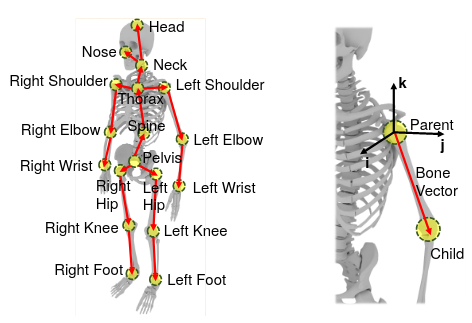
\includegraphics[height=4cm, width=7cm]{skeleton.png}
%    \caption{\todo{remove if > 3 pages} Hierarchical human representation. Left: 3D key-points organized in a kinematic tree where red arrows point from parent joints to children joints. Right: Zoom-in view of a local coordinate system, source ~\cite{Li_2020_CVPR}}
%    \label{skeleton}
%\end{figure}

%Every parent node has attached a local coordinate system. For $\textbf{p}^{parent(i)}$ local coordinate system is represented by the rotation matrix $\textbf{R}^i = [\textbf{i}^i, \textbf{j}^i, \textbf{k}^i]$, which is used to transform the bone vector into the local coordinate system with the following equation:

%$$\textbf{b}_{local} ^{i} = \textbf{R}^{i\textbf{T}}(\textbf{p}^{child(i)}-\textbf{p}^{parent(i)})$$

%which is for convenience transformed into spherical coordinates $\textbf{b}_{local}^i = (r_i, \theta _i, \phi _i)$.

The overall algorithm can be seen in ~\ref{alg1}.

\begin{algorithm}
    \SetKwInOut{Input}{input}
    \Input{Initial population of 3D joints $D_{old}=\{\textbf{p}\}_{i=1} ^N$, noise $\sigma$, number of generations $G$}

    $D_{new} = D_{old}$

    \For{i=1:G}{
        Parents=Sample($D_{new}$)

        Children=NaturalSelection(Mutation(Crossover(Parents)))

        $D_{new} = D_{new} \cup Children$
    }
    return $D_{new}$
    \caption{Data evolution}
    \label{alg1}
\end{algorithm}

With algorithm ~\ref{alg1} we create 2D-3D pairs for teaching the model to map from 2D to 3D.
Crossover is implemented as a random exchange of sub-trees of bones.
The mutation operator perturbates the local orientation of one bone vector for a certain degree.
Mutation can easily make an invalid pose, therefore we use natural selection to remove invalid poses.
Natural selection is implemented using a function which indicates which pose is invalid
and gives that pose a value of $-\infty$ making it unable to be selected into the new generation.
This function uses the prior angle constraints defined from ~\cite{Akhter_2015_CVPR}.
Both mutation and crossover can be seen in Fig. ~\ref{evolved}

\begin{figure}
    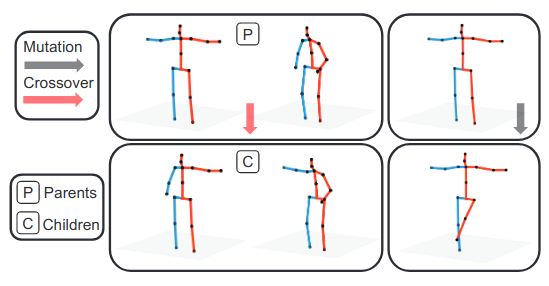
\includegraphics[height=5cm, width=8.5cm]{evolution.png}
    \caption{Examples of evolutionary operation. Crossover and mutation take two and one random samples respectively to synthesize novel human skeletons. In this example the right arms are selected for crossover while the left leg is mutated., source ~\cite{Li_2020_CVPR}}
    \label{evolved}
\end{figure}

\subsection{Miscellaneous}

%In addition to the approaches above, we have combined them with a variety of further techniques.
%As the official PyTorch documentation recommends loading in the data in the range of [0, 1],
%we have tried [0, 1]-normalization instead of the original z-standardization.
%Preliminary experiments showed that this does not improve the score, hinting at a slight decrease
%which is why it was not further used.

Although ensemble methods were not allowed, using dropout layer were an exception.
Hence, we have experimented using a dropout layer after the heatmaps and the feature extraction part,
however it did not improve our score compared to our best model.

Before evaluating the SemGCN architecture to lift our 2D joint predictions to 3D, we explored the idea of utilizing a de-noising autoencoder as a refinement step to our 3D joint predictions.
We borrowed this idea from the authors \citeauthor{ghosh_learning_2017} \cite{ghosh_learning_2017} which use this component to adjust unfeasible poses from human motion predictions.
After some testing of this idea, we learned about the SemGCN architecture which seemed more promising and hence stopped further exploration.

%After initial test runs of the SemGCN architecture, we noticed a bottleneck stemming from our 2D joint predictions
%when compared to training on the ground truth 2D H36M data.
%As we previously simply dropped the last axis of our 3D predictions to create the 2D input,
%we thought if we train the backbone to predict 2D joint locations only, accuracy might improve.
%Having tried both methods with no improvement, we concluded that there is no performance
%gain in varying these two approaches.
%Exploiting SemGCN's resemblance to the human skeleton, a comparison is also made between using 2D and 3D joints
%as input data.
%In the latter case the SemGCN would act as a final refinement step.

Both, the de-noising autoencoder and the SemGCN, focus more or less on capturing the overall human pose composition.
This idea was already explored in a different way by \citeauthor{sun_compositional_2017} \cite{sun_compositional_2017}
where they proposed a loss function which incorporates information of the skeleton.
Instead of calculating the loss as $\sum_{k=1}^K ||\tilde{\mathbf{J}}_k-\mathbf{J}_k||_1$ which only considers the joint position they proposed a loss which incorporates bone lengths.
Given a bone, $\mathbf{B}_k=\mathbf{J}_{parent(k)}-\mathbf{J}_k$, the loss is formulated as $\sum_{k=1}^K ||\tilde{\mathbf{B}}_k-\mathbf{B}_k||_1$.
Even tough this should e.g. avoid unrealistic poses, incorporating this loss did not improve our score.


\section{Evaluation}
We evaluate models for 10 to 30+ hours, starting with a learning rate of 0.0001 and decaying it once the loss seems to have converge.
For our final model we trained for 65 epochs on both the MPII and the H36M dataset simultaneously with a batch size of 16. Here, the learning rate was decayed by 0.1 after 55, 60, and 65 epochs.

%\todo{In the evaluation section you should describe the experiments that support the claims of the story of your report. For example, if you previously said ``We propose to combine model A with component B which leads to improved accuracy.'' you should back this up with experimental evidence here. Typically, this means that you should show the performance of model A with and without component B. May be your method warrants other kinds of such ablation studies, which you might include and describe here.}


\begin{table}[h!]
    \caption{Ablation study on the progression of the Mean Per Joint Position Error (MPJPE) metric.
    The score denotes the performance on the test set. Values with $*$  denote the performance on the validation set.
    Data augmentation (A), Bone Loss (B), %Backbone Completely Frozen (C),
    Evolved Data (D), Extra Data (E), Remove Joint Grouping (G), Higher Resolution (H),
    Integral Heatmap Regression (I), Data occlusion (O),
    Ground Truth Pre-Training (P), 3D-Regression (R), SemGCN Head (S),
    Last Layer Unfrozen (U), 3D SemGCN Input (3)}

    \label{tab:ablation}
    \centering
    \begin{tabular}{|| c | c | c ||}
        \hline
        \textbf{Backbone} & \textbf{Extensions} & \textbf{MPJPE}$_{test}$ \\
        \hline\hline
        AlexNet           & R                   & 141.50                  \\
        \hline
        AlexNet           & O                   & $84.50$                 \\
        \hline
        ResNet50          & I                   & $72.15$                 \\
        \hline
        ResNet50          & I,O                 & $63.01$                 \\
        \hline
        ResNext101        & I,O,A               & $54.14$                 \\
        \hline
        ResNext101        & I, O, A, S, 3       & $57.43$                 \\
        \hline
        ResNet152         & I,O,A,H,E           & $50.94$                 \\
        \hline
        ResNext101        & I,O,A,H,E           & $46.48$                 \\
        \hline
        ResNext101        & I,O,A,B             & $54.60^*$               \\
        \hline
        \hline
        SemGCN            &                     & $66.87^*$               \\
        \hline
        SemGCN            & P                   & $60.08^*$               \\
        \hline
        SemGCN            & P, U                & $54.12^*$               \\
        \hline
        SemGCN            & P, U, G             & $46.05^*$               \\
        \hline
        SemGCN            & P, U, G, D          & $45.68^*$               \\
        \hline
    \end{tabular}
\end{table}

\subsubsection*{Synthetic occlusion}
Using the given sample code with the AlexNet as the backbone of the model synthetic occlusion
gives an impressive improvement to the score lowering it by 40.28\%.

\subsubsection*{Model backbone}
A stronger backbone plays a significant role when it comes to improving the score.
Using the ResNet50 with integral heatmap regression improved the score from the initial model by 49.01\%.
Adding synthetic occlusion to that gives a score which has 12.69\% lower MPJPE on the test set.
Furthermore, using an even more powerful backbone such as ResNext101 with integral heatmap regression, synthetic occlusion and standard augmentation improved the model to a score of 54.14 MPJPE.
One can compare using ResNext101 to ResNet152 with identical extensions
as shown in ~\ref{tab:ablation} to see that ResNext101 improves the score by 3.91\%.

\subsubsection*{Larger image size/depth resolution/dataset} These three extension were added simultaneously and, thus it is difficult to tell which one impacted the score by how much.
However, is was clear that these extensions have a positive impact \cite{sun_integral_2018-1}.
In our case, we could improve our performance on the MPJPE from 54.14 to 46.48 which is a decrease by around 14\%.
Regarding the changes to the image size, the resolution was increased from 256 x 256 to 288 x 384.
For the depth resolution/the amount of heatmaps produced per joint, the value was increased from 64 to 72.
As we wanted to utilize all the resources available to us, the final model was trained on the training and validation set of both the MPII and the H36M.


\subsubsection*{SemGCN}
In regards to the SemGCN model, only the scores of the z-axis matter as the other 2D input is the ground truth.
Thus, the following error scores for the SemGCN are not directly comparable to the others. Our first experiments showed that when not pre-training the SemGCN model on ground truth data,
it is able to achieve a validation score of 66.87.
This can be brought down to 60.08 by incorporating pre-training.
%The best variant making use of pre-training on ground-truth data achieves a validation error of 54,
%while not pre-training achieves 66.
As a next step we then analyzed the effect of unfreezing the last layer of the backbone which
achieves a score of 54.12.
Unfreezing the SemGCN without any pre-training on the other hand got an error of around 65.5.
This could be explained due to the fact that we stop training the model if it seems to perform badly
early on, which is the case for non-pre-trained models as these take longer to train.
%This best pre-trained SemGCN leaves the last layer unfrozen, while freezing
%the backbone completely achieved a validation error of 60.08 when using a pre-trained model.
Like previously mentioned, we compare different ways of adding the missing 17th joint.
%ranging from simple concatenation and group removing
%to more sophisticated grouping with other joints and reordering.
Surprisingly the grouping methods even in combination with joint reordering perform similarly bad
with scores around 60 using pre-trained models. Removing the grouping altogether seems to prove most useful, being able to get a validation error of 46.05.
%This holds for the case where we change the architecture to not consider grouping as well as when
%we simply change the group size to 1 instead of 2.
%This might be explained due to the model's robustness
%and the possibility that few of the joints make up for most of the information lying underneath.

%\todo{I'd just leave out going into detail for End to End Models selling it as the same thing for both
%and maybe in passing mention that we did not
%validate them all too much as the SemGCN didn't perform too well already.
%Or we can have SemGCN (S) as an extension for the ablation study and add it under ResNext}


\begin{figure}
    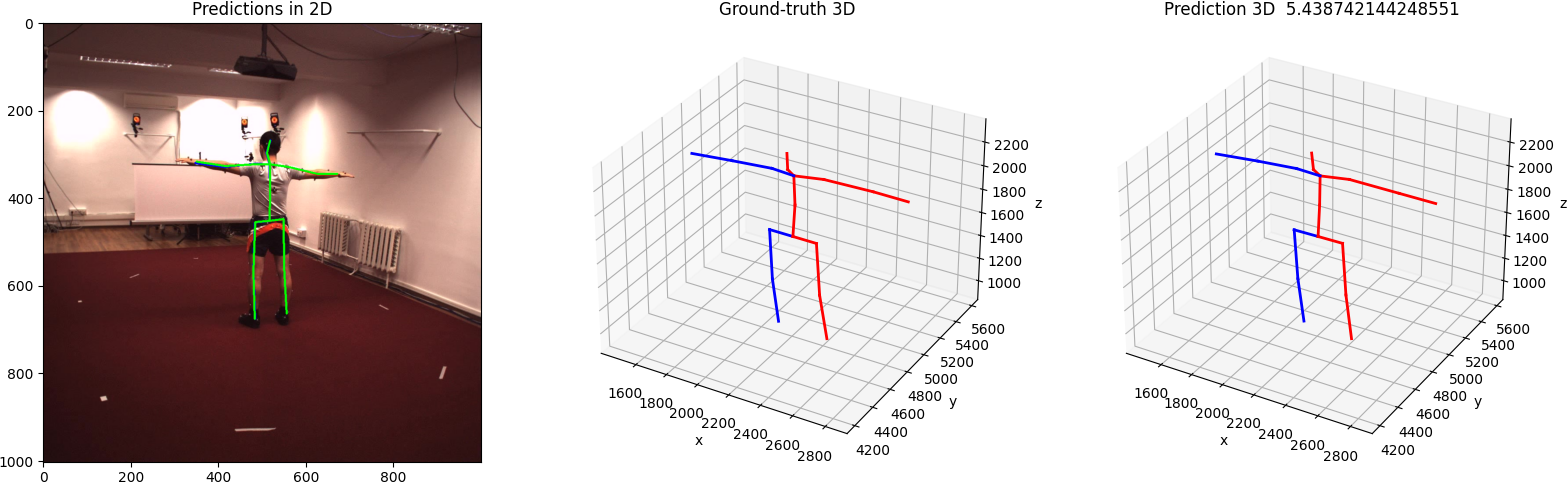
\includegraphics[width=\columnwidth]{figures/tensorboard_1}
    \caption{Visualization of a random sample of the H36M Dataset.
    Left: Input picture with overlaid 2D ground truth and prediction; Middle: ground truth; Right: Our prediction}
    \label{tensorboard}
\end{figure}

\section{Discussion}
In section \ref{method} and \ref{approach} we showcased that we explored a wide variety of approaches in order to solve the task of HPE.
In comparison to section \ref{method}, section \ref{approach} presented approaches which performed worse than our best model.
We think that the main reason for this was the inability of our backbone to predict close to the 2D ground truth which hindered the presented methods to show their full potential.



\section{Conclusion}
%Conclude your report with a brief summary. This can be very short, i.e. 2-3 sentences.
In this paper we compare a variety of different architectures and techniques for the
task of 3D human pose prediction on the H36M dataset \cite{h36m_pami}.
We provide an extensive benchmark study analyzing direct image-to-3D-joint prediction
as well as image-to-2D-joint prediction with a final 3D regression.

Our best model makes use of augmentation and occlusion, volumetric heatmap regression in combination with
a pretrained ResNext101 backbone and is able to beat the state of the art in the monocular, single frame H36M benchmark~\cite{h36msinglecam, Li_2020_CVPR}. % \todo{reference for score? }

% maybe add another sentence about our best 3D regressor SemGCN model

%\clearpage



\bibliographystyle{ACM-Reference-Format}
\bibliography{bibliography}

\end{document}
